\documentclass[a4paper]{article}
\usepackage[pdftex]{graphicx,color}  % ab: for xfig pdf export
%\usepackage{showframe}
% minted
\usepackage{minted}
\usemintedstyle{lovelace}
\definecolor{bg}{rgb}{0.95,0.95,0.95}
\definecolor{bg_shell}{rgb}{0.95,0.95,1.00}
%\newminted[python]{python}{bgcolor=bg, frame=lines}
\newminted[python]{python}{frame=lines}
%\AfterEndEnvironment{minted}{\par\noindent}
%\makeatletter
%\patchcmd{\minted@colorbg}{\noindent}{\medskip\noindent}{}{}
%\apptocmd{\endminted@colorbg}{\par\medskip}{}{}
%\makeatother




%\addtolength{\topmargin}{-2cm}
\addtolength{\textheight}{1cm}
%\addtolength{\textwidth}{1cm}
%\addtolength{\oddsidemargin}{-0.5cm}



\title{Techblog-to-be? --- The Expertmaker Accelerator\\[1ex]\large{Processing One Billion Lines of Data per Second on a
  Single PC}\\\Large{--- Abstract ---}}

\author{A.\,Berkeman, C.\,Drougge, and S.\,H\"orberg}
\date{}

\begin{document}
\maketitle
\thispagestyle{empty}

\begin{figure}[h]
  \centering
  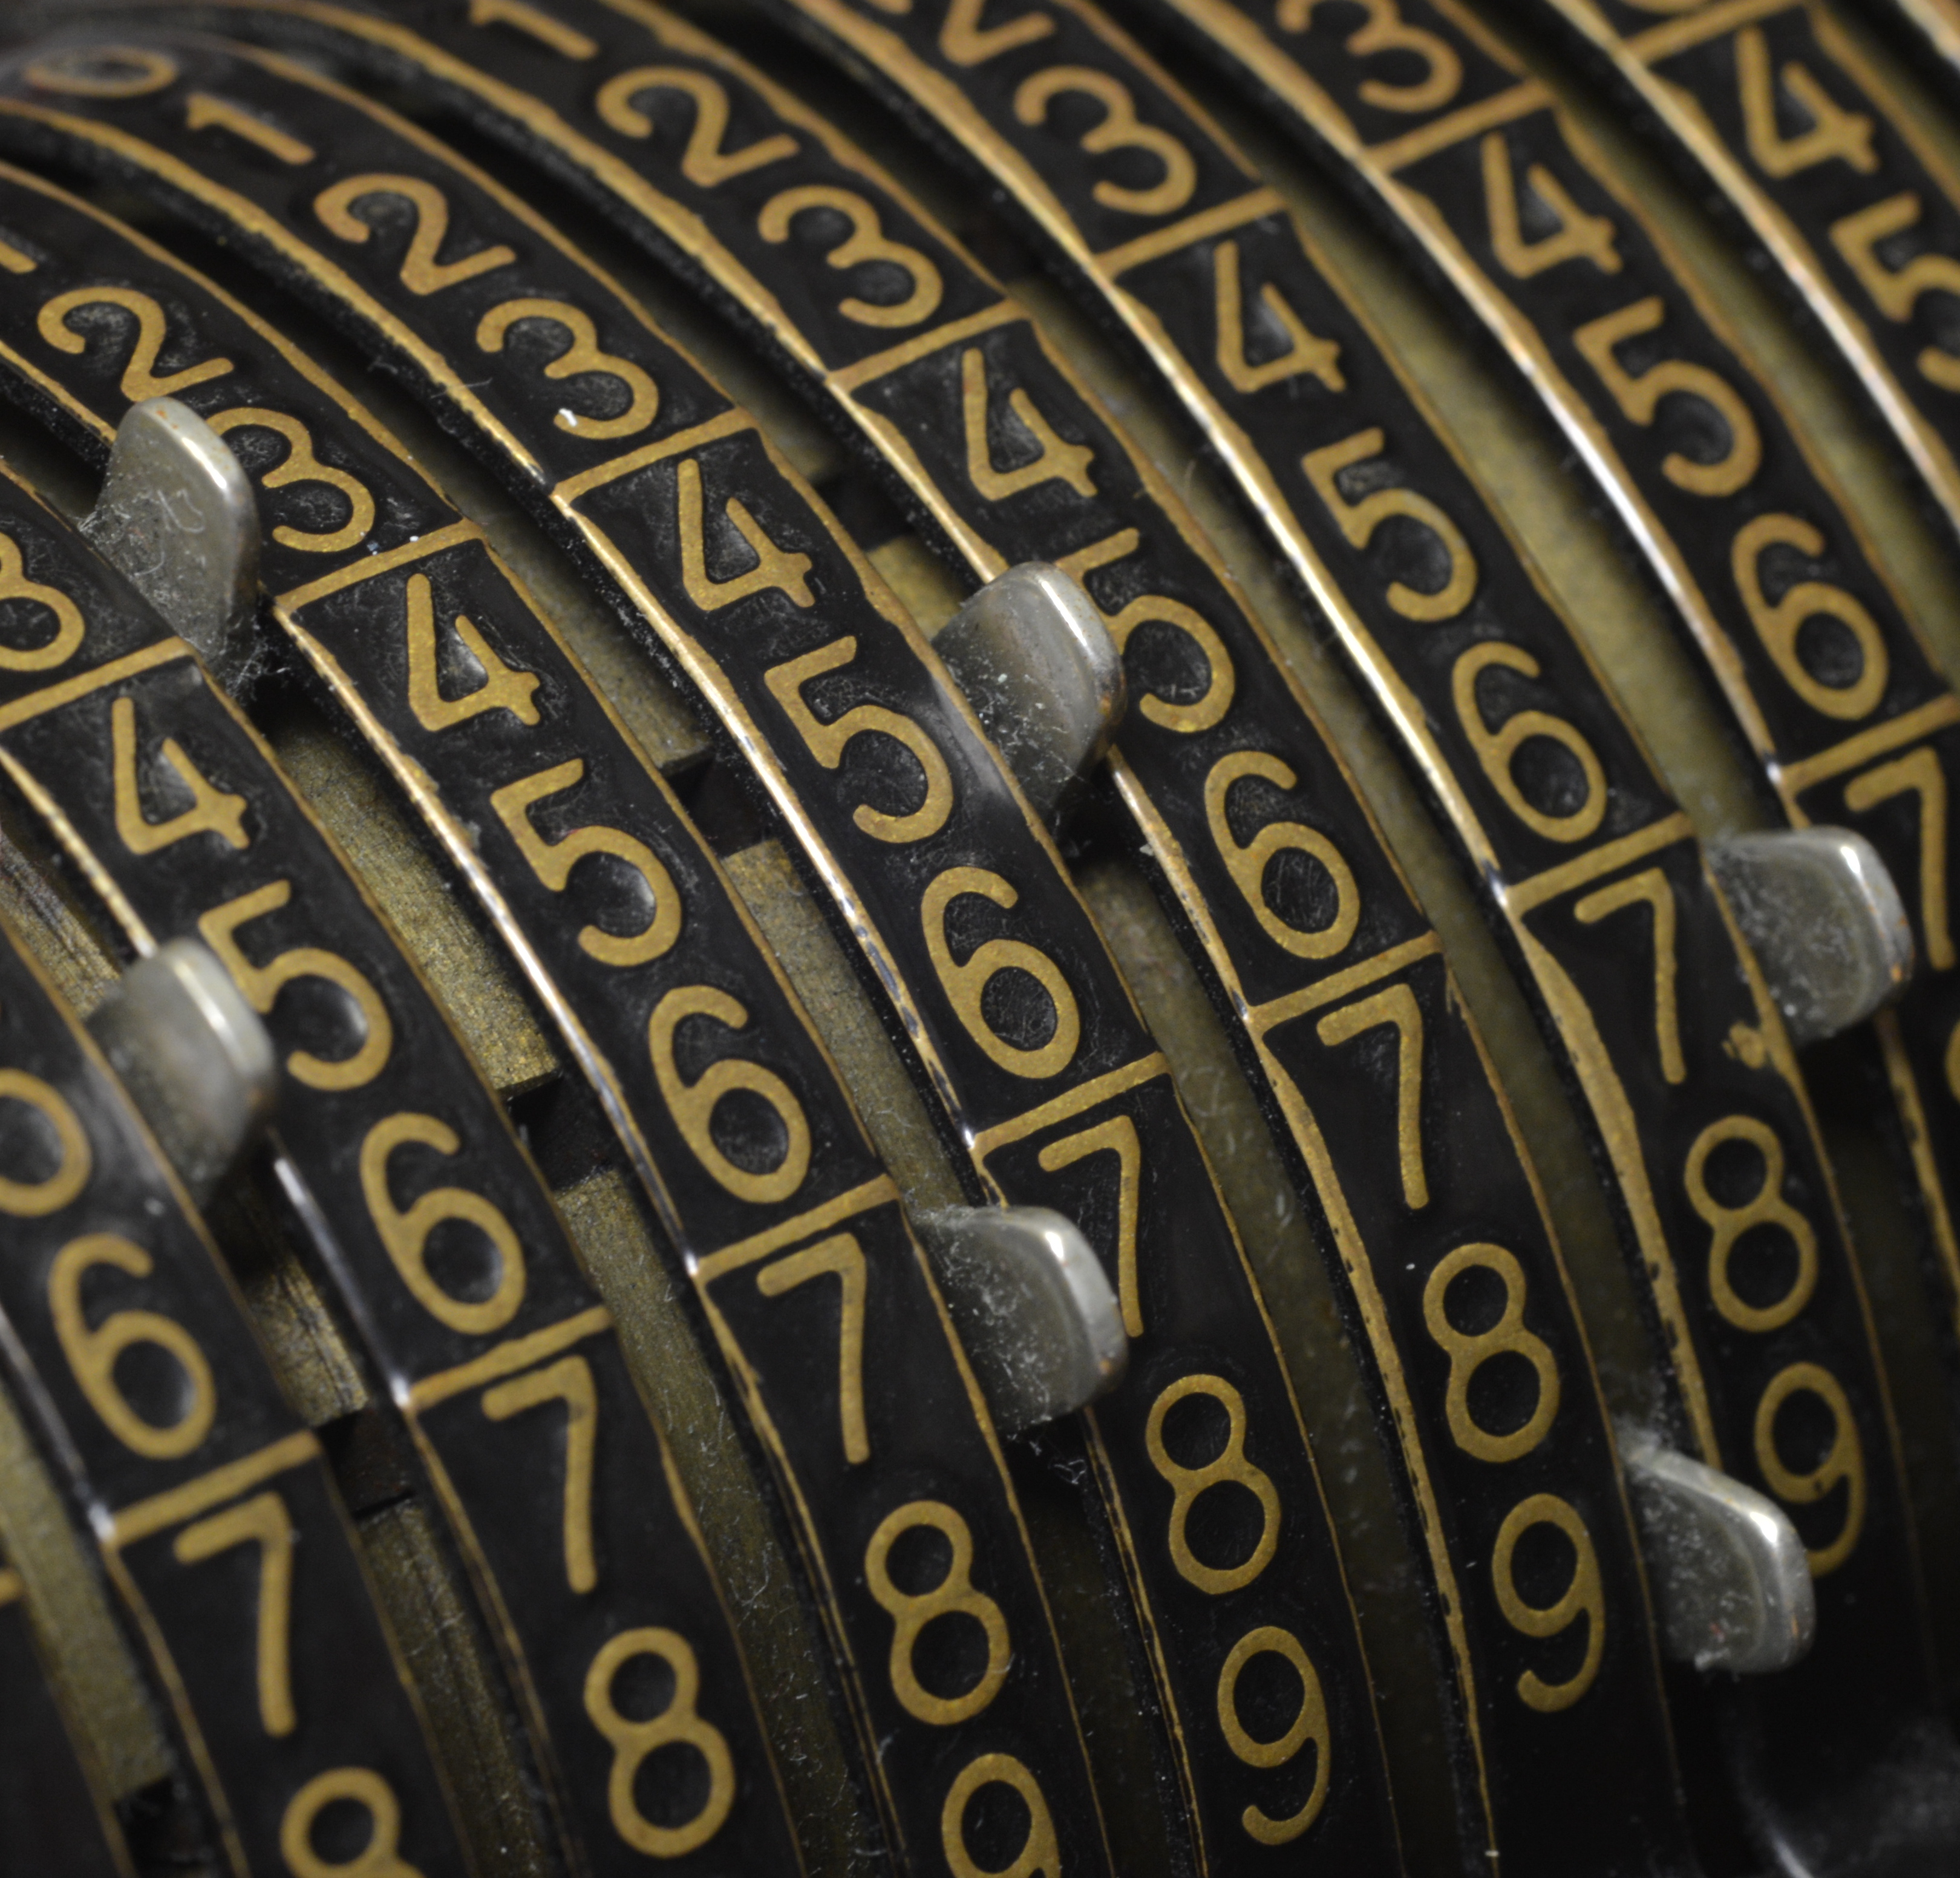
\includegraphics[width=11cm]{odhner_square.jpg}
\end{figure}

%% \begin{figure}[h]
%%   \begin{center}
%%     \input{figures/test.pdftex_t} %the difference is just this part
%%     \caption{caption here}
%%     \label{figure:example}
%%   \end{center}
%% \end{figure}



% Your 1-page abstract should include:

% Motivation: Why do we care about the problem and the results?

% Problem statement: What problem are you trying to solve? What is
%   the scope of your work (a generalized approach, or for a specific
%   situation)?

% Approach: How did you go about solving or making progress on
%   the problem? Did you use simulation, analytic models,
%   prototype construction, or analysis of field data for an
%   actual product? What was the extent of your work (did you look
%   at one application program or a hundred programs in twenty
%   different programming languages?) What important variables did
%   you control, ignore, or measure?

% Results: What's the answer?
%   Conclusions: What are the implications of your answer? Is
%   it going to change the world (unlikely), be a significant
%   ``win'', be a nice hack, or simply serve as a road sign
%   indicating that this path is a waste of time (all of the
%   previous results are useful). Are your results general,
%   potentially generalizable, or specific to a particular
%   case?
            

%% \emph{
%%  teaser om hur coola grejer man kan göra innan vi börjar med triviala
%%  exempel...  ``Så, för att förstå hur det är möjligt måste vi börja
%%  med...'', typ
%% }\\

%% \emph{Maste namna workspace eller om det heter workdir}\\

%% \emph{Maste namna python}\\


%% \subsection*{What It Is}
%% The Expertmaker Accelerator is a tool for processing big data.  It has
%% a small footprint and low overhead, and provides a number of
%% interesting features, most notably very fast data access and a novel
%% scheme to store, retrieve, and reuse computations.  It has been used
%% in commercial projects since 2012.

%% \subsection*{Background}
%% vad den anvants till, hur den utvecklats osv

%% \subsection*{Motivation and Approach}
%% Processing big data is potentially both time consuming and resource
%% hungry.  This is addressed in the Accelerator design by the following
%% two principles:
%% \begin{itemize}
%% \item[1.] Modern computers are very powerful.\\ The Accelerator has
%%   very vast data streaming from disk to CPU cores.  Critical parts are
%%   written in the C programming language, and effort has been spent to
%%   come close to the theoretical performance limits set by modern
%%   hardware.
  
%% \item[2.] Results are valuable, they should be easy to retrieve and
%%   re-use.\\ The Accelerator connects each computed result to the
%%   source code that was running, the input data used, and the set of
%%   input parameters.  This connection makes it possible for the
%%   Accelerator to automatically retrieve results instead of
%%   re-computing them, which saves time.  It also brings full
%%   transparency in that all work can be trivially traced back to its
%%   origins.
%% \end{itemize}



















%%%%%%%%%%%%%%%%%%%%%%%%%%%%%%%%%%%%%%%%%%%%%%%%%%%%%%%%%%%%%%%%%%%%%%%%%%%%%%%%
\clearpage
\section{Executing Code: Jobs}
The basic operation of the Accelerator is to execute small programs
called \textsl{methods}.  A method is, simply put, a python program
that instantates one or more special functions.



\subsection{Basic Job Running:  ``Hello, World''}

Let's begin with a simple ``hello world'' program.  We create a method
with the following contents
\begin{python}
def synthesis():
    return "hello world"
\end{python}
This program does not take any input parameters.  It just returns a
string and exits.

When execution of the method is completed, a single link, called a
\texttt{jobid} is the only thing that is returned to the user.  The
jobid points to a directory where the result from the execution is
stored, together with all information that was needed to run the job
plus some profiling information.

If we try to run the job again it will not execute, simply because the
Accelerator remembers the job has been run in the past.  Instead of
running the job again, it immediately returns the jobid pointing to
the previous run.  This means that from a user's perspective, there is
no difference between job running and job result recalling!  In order
to have the job executing again, we have to change either the source
code or input parameters.

Figure~\ref{fig:execflow-hello-world} illustrates the dispatch of the
\texttt{hello\_world} method.  The created jobid is called
\texttt{job\_0}, and corresponding directory information is shown in
green.  The job directory contains several files, of which the most
important ones right now are
\begin{itemize}
  \item[] \texttt{setup.json}, which contains job information; and
  \item[] \texttt{result.pickle}, that contains the returned data.
\end{itemize}

\begin{figure}[h!]
  \begin{center}
    \input{figures/job0.pdftex_t}
    \caption{A simple hello world program.}
    \label{fig:execflow-hello-world}
  \end{center}
\end{figure}

\clearpage





\subsection{Linking Jobs}
Assume that the job that we just run was computationally expensive,
and that it returned a result that we'd like to use as input to further
processing.

To keep things simple, we create a method that just reads and prints
the result from the previous job to \texttt{stdout}.  We create a new
method \texttt{print\_result}, that goes like this

\begin{python}
import blob
  
jobids = {'hello_world_job',}

def synthesis():
    x = blob.load(jobid=jobids.hello_world_job)
    print(x)
\end{python}

This method expects the \texttt{hello\_world\_job} input parameter to
be provided at execution time.  The method then reads the result from
the provided jobid and assigns it to the variable \texttt{x}, which is
then printed to \texttt{stdout}.  Note that this method does not
return anything.  Figure~\ref{fig:execflow-print-result} illustrates
the situation.  Note the direction of the arrow - The second job,
\texttt{job\_1} had \texttt{job\_0} as input parameter, but
\texttt{job\_0} does not know of any jobs run in the future.

\begin{figure}[h!]
  \begin{center}
    \input{figures/job0job1.pdftex_t}
    \caption{Jobid \texttt{job\_0}, is used as input to the
      \texttt{print\_result} job.}
    \label{fig:execflow-print-result}
  \end{center}
\end{figure}



\clearpage





\subsection{Job Parameters}


We've seen how jobids from completed jobs can be used as input to new
ones.  This is one of three kinds of input parameters that a job can
take.  Here the input parameters are summarised:
\begin{itemize}
  \item[] \texttt{jobids}, a set of identifiers to previously executed jobs.
  \item[] \texttt{options}, a dictionary of options;
  \item[] \texttt{datasets}, a set of input \textsl{datasets}, explained later; and
\end{itemize}
See Figure~\ref{fig:execflow}.

\subsubsection{jobids}
Any number of jobids can be supplied as input to a job.  For example
\begin{python}
  jobid = {'sales_stats', 'overhead_stats',}
\end{python}

\subsubsection{options}
Options are supplied as a dictionary and is very flexible in typing.  For example
\begin{python}
  options = dict(
    name = 'alice',
    defaultnames = set('alice', 'bob'),
    param1 = 1,
    param2 = float,
  )
\end{python}
Here, values are defaults, so \texttt{param1} is default set to 1,
while a floating point value must be supplied to \texttt{param2}.

\subsubsection{datasets}
Datasets will be described in more details later, but the
\texttt{datasets} parameter is similar to the \texttt{jobids}
parameter.

\begin{figure}[h!]
  \begin{center}
    \input{figures/execflow.pdftex_t}
    \caption{Execution flow of a method.  The method takes optionally
      three kinds of parameters: \texttt{options}, \texttt{jobids},
      and \texttt{datasets}.}
    \label{fig:execflow}
  \end{center}
\end{figure}

\clearpage



\subsection{Jobs in more Detail}
A recap and bit more flesh on the bones regarding jobs
\begin{itemize}
\item[1.]  Data and metadata relating to a job is stored in a job directory.
\item[2.]  This job directory is pointed to by a jobid.
\end{itemize}
The files stored in the job directory at dispatch are complete in the
sense that they contain all information required to run the job.  So
the Accelerator job dispatcher actually just creates processes and
points them to the job directory.  Then, the processes have to go
figure out the rest by themselves.

A running job has its \textsl{current working directory} pointing into
the job directory, so any files created (plus return values) by a job
will by default be stored in the job's directory.

When the job completes, the files are updated with profiling
infomation, such as execution time spent in single and parallel
processing modes.

All code that is directly related to the job is also stored in a
compressed archive.  This arhive is typically limited to the method's
source, but the code may have manually added dependencies to any other
files, and in that case these are added too.  This way, source code
and results are always connected and conveniently stored in the same
directory for future reference.
\begin{itemize}
\item[3.]  Unique jobs are only executed once.
\end{itemize}
Among the meta information stored in the job directory is a hash
digest of the method's source code (including manually added
dependencies).  This hash together with the input parameters is used
to figure out if a result could be re-used instead of re-computed.  In
the next section we'll see how this feature brings a number of
advantages.
\begin{itemize}
\item[4.]  Jobs may link to eachother using jobids.
\end{itemize}
Which means that jobs may share results and parameters with eachother.
\begin{itemize}
\item[5.]  Jobs are stored in workdirs.
\item[6.]  There may be any number of workdirs.
\end{itemize}
This adds a layer of ``physical separation''.  All jobs relating to
importing a set of data may be stored in one workdir, perhaps named
\texttt{import}, and development work may be stored in a workdir
\texttt{dev}, etc.  Jobids are created by appending a counter to the
workdir name, so a job \texttt{dev\_42} may access data in
\texttt{import\_3}, and so on, which helps manual inspection.
\begin{itemize}
\item[] Jobs may dispatch other jobs.
\end{itemize}
It is perfectly fine for a job to dispatch any number of new jobs, and
these jobs are called \textsl{subjobs}.


to a recurse limit.  The API for dispatching job
xxxit\clearpage






\subsection{Advantages}
Let's have a short summary of what we've seen so far and what it
means.  The fact that jobs may link to eachother combined with the
fact that jobs may only be executed once brings a number of
advantages, of which two really stand out.
\begin{itemize}
\item[1.] All previous results will be available immediately upon
  request.  This means that we can speed up development and execution
  time, since we do not ever need to recompute anythin.  This is
  particularly advantageous when using an incremental design strategy,
  designing one job at a time.
\item[2.] All previous results are stored and bookkept, so there is a
  full log of which job that was run and when, which input data the
  job used and what the job parameters were.  This means that the way
  from input data to output result is fully transparent and easy to
  follow.  Much less risk of mixing up files and results.
\end{itemize}

\clearpage





\section{Datasets: Storing Data}

The \texttt{dataset} is the Accelerator's default storage type for
small or large quantities of data.  Datasets are created by methods
and stored in job directories, just like any job result.

Data is stored in a row-column format, and is typically sliced into a
fixed number of slices to allow efficient parallell access.
Furthermore, datasets may be \textsl{hashed}, so that slicing is based
on the hash value of a given column.  In many practical applications,
hashing makes parallel processes independent, minimising the need for
complicated merging operations.



\subsection{Importing Data}

Let's have a look at the common operation of \textsl{importing},
i.e.\ creating a dataset from a file.  See
figure~\ref{fig:dataset_csvimport}.

\begin{figure}[h!]
  \begin{center}
    \input{figures/dataset_csvimport.pdftex_t}
    \caption{caption here}
    \label{fig:dataset_csvimport}
  \end{center}
\end{figure}

\noindent The standard method, \texttt{csvimport}, is used to parse a
pletoria of ``comma separated values''-file format and store as a
dataset.  The method takes several input options, where the file name
is mandatory.  The created dataset is stored in a job, and the name of
the dataset will by default be the jobid plus the string
\texttt{default}.  For example, if the \texttt{csvimport} jobid is
\texttt{imp\_0}, the dataset will be referenced by
\texttt{imp\_0/default}.  In this case, and always when there is no
ambiguity, the jobid alone (\texttt{imp\_0}) could be used too.

\clearpage




\subsection{Linking Datasets, Chaining}

Just like jobs, a key feature is that datasets can be linked to
eachother.  Assume that we've just imported \texttt{file1.txt} into
\texttt{imp\_0/default}.  Now, there is more data like it stored in
\texttt{file2.txt}, we can import the latter file and supply a link to
the previous dataset, see figure~\ref{fig:dataset_csvimport_chain}.

\begin{figure}[h!]
  \begin{center}
    \input{figures/dataset_csvimport_chain.pdftex_t}
    \caption{caption here}
    \label{fig:dataset_csvimport_chain}
  \end{center}
\end{figure}

\noindent If we look at the datasets only we have a situation like in
figure~\ref{fig:dep_dataset_csvimport_chain}.  The second import was
fed with the input dataset from \texttt{job\_0}, and this link is
represented by the arrow in the image.

\begin{figure}[h!]
  \begin{center}
    \input{figures/dep_dataset_csvimport_chain.pdftex_t}
    \caption{caption here}
    \label{fig:dep_dataset_csvimport_chain}
  \end{center}
\end{figure}

\noindent The \texttt{job\_1} dataset reference can now be used to
access all data imported from both files.

Linking datasets containing related content is called
\texttt{chaining}, and this is particularly convenient when dealing
with data that grows over time.  A typical kind is log data, and it
could be a log of transactions, user interactions, etc.

\clearpage




\subsection{Multiple Datasets in a Job}

Datasets are created by methods and stored in job directories.
Typically, a method creates a single dataset in the job directory, but
there is no limit on how many datasets that could be stored in a
single job directory.  This leads to some interesting applications.

One situation where it is convenient to create multiple datasets in a
job is when separating data into subsets based on some condition.  For
example, assume that we want to separate a dataset into two disjoint
datasets based on a column storing a boolean value.  See
Figure~\ref{fig:dep_dataset_csvimport_chain}.

\begin{figure}[h!]
  \begin{center}
    \input{figures/filter_dataset.pdftex_t}
    \caption{caption here}
    \label{fig:dep_dataset_csvimport_chain}
  \end{center}
\end{figure}

\noindent The figure show how \texttt{job\_1} has created two
datasets, \texttt{job\_1/True} and \texttt{job\_1/False}, based on the
input dataset \texttt{job\_0/default}.  A third job, \texttt{job\_2}
is then accessing the \texttt{job\_1/True} dataset.


%% Short repetition on the direction of the arrow.  \texttt{job\_1}
%% filtered the \texttt{dataset} from \texttt{job\_0}.  So if we take a
%% look at \texttt{job\_1} and wonder where the input data is, we just
%% follow the link back to \texttt{job\_0}.  If this job is an import, it
%% will hold the name of the file that was imported.  If not, it will
%% link back to another job, and so on, all the way down to the source of
%% the dataset.  So there is full tracking and easy observability of
%% everything that relates to job execution in the Accelerator.

\noindent Let us look at an example of when such dataset splitting
makes sense, and how it relates to the design methodology that the
Accelerator is based upon.  Assume that we have a (perhaps large)
dataset that we want to split into, say, a training set and a
validation set.  Even if one set is small, it makes sense to split the
dataset into two disjoint sets.  This way, we ``physically'' separate
the data into two sets, while keeping all the data in the same place.
This is good for transparency reasons, and any method following the
split may iterate over both subsets to read the complete data.

\clearpage




%% \subsection{Understanding Datasets}
%% A \texttt{dataset} is a storage of a matrix of data.  It has a number
%% of rows and a number of columns.  The columns have names and types.
%% In order to have fast parallell execution, the columns are split into
%% a fixed number of \textsl{slices}.



\subsection{Adding New Columns to a Dataset}
We have seen how easy it is to add more lines to data to a dataset
using chaining - the only thing that needs to be done is to set a
link, so the overhead is minimal.

Now we'll see that is it equally simple to add new columns to an
existing dataset.  Adding columns is also a common operation and the
Accelerator handles it efficiently using links.

The idea is very simple.  Assume that we have a ``source'' dataset to
which we want to add a new column.  We create a new dataset containing
\textsl{only} the new column, and while creating it we instruct the
Accelerator to link to source dataset as its \textsl{parent}.  The
naming might not be perfect, but there it is.

Accessing the new one-column dataset will transparently access all the
data in the source dataset too, making it indistinguishable from a
single dataset.  See Figure~\ref{fig:dep_dataset_append_column}.

\begin{figure}[h!]
  \begin{center}
    \input{figures/dataset_append_column.pdftex_t}
    \caption{caption here}
    \label{fig:dep_dataset_append_column}
  \end{center}
\end{figure}

\clearpage





\subsection{Dataset Internals}

On a high level, the dataset stores a \textsl{matrix} of rows and
columns.  Each column is represented by a column name, and all columns
have the same number of rows.  Columns are typed, and there is a wide
range of types available.

The dataset is further split into disjoint slices, where each slice
holds a unique subset of the dataset's rows.  Slicing makes simple but
efficient parallel processing possible.  See Figure~\ref{fig:slices}.
The number of slices is set initally by the user, and all workdirs
that are used together in a project must use the same number of
slices.

On a low level, there is one file stored on disk for each slice and
column.  A job that needs to read only a subset of the total number of
columns may open and read from the relevant files only.

A technical note: If the number slices is large and files are small,
there will be a signinficant overhead from disk \texttt{seek()} if
using rotating disks.  The Accelerator mitigates this by using single
files with seek-indexing when appropriate.


\begin{figure}[h!]
  \begin{center}
    \input{figures/slices.pdftex_t}
    \caption{Dataset internals}
    \label{fig:slices}
  \end{center}
\end{figure}

\clearpage



\section{Datasets: Working with Data}

In this section, we'll have a look at how to access the data stored in
a dataset, and how to take advantage of slicing to have parallel
processing.

\subsection{Iterator Basics}

Assume that we have a dataset with a column containing movie titles
named \texttt{movie}, and we want to know the ten most common titles.
Consider the following complete code example
\begin{python}
from collections import Counter
datasets = ('source',)

def synthesis():
    c = Counter(title for title in datasets.source.iterate(None, 'movie'))
    print(c.most_common(10))
\end{python}
This will print the ten most common titles and their
frequencies in the \texttt{source} dataset.  The code will run on a
single CPU core, because of the \texttt{synthesis} function, which is
called only once.  The \texttt{iterate} (class-)method therefore has
to read through all slices in a serial fashion, and this is instructed
by the first \texttt{None}-parameter.



\subsection{Parallel Execution}
The Accelerator is much about parallel processing, and since datasets
are slices, we can modify the above program to execute in parallel by
doing the following modification
\begin{python}
def analysis(sliceno):
    return Counter(title for title in datasets.source.iterate(sliceno, 'movie'))

def synthesis(analysis_res)
    c = analysis_res.merge_auto()
    print(c.most_common(10))
\end{python}
Here, we run \texttt{iterate} inside the \texttt{analysis()} function.
This function is forked once for each slice, and the argument
\texttt{sliceno} will contain an integer between zero and the number
of slices minus one.  The returned value from the analysis functions
will be available as input to the synthesis function in the iterator
variable \texttt{analysis\_res}.  It is possible to merge the results
explicitly, but the iterator comes with a rather magic method
\texttt{merge\_auto()} which merges the results from all slices into
one based on the data type.  It is rather advanced, and can handle for
example \texttt{Counter}s, \texttt{set}s, and composed types like
\texttt{set}s of \texttt{Counter}s, and so on.

\clearpage


\subsection{More on the Iterator}
The iterator can run on chained datasets and there are various stop
conditions: stop after a certain number of datasets, stop at a certain
dataset, stop at another jobs input parameters.

It is possible to iterate over a range of lines in a dataset

hashlabel
translators/filters
callback
multi-user
urd - how?

rehasha dataset istället för enorm reduce!


dataset\_separate\_by\_bool i agg-projektet.  Fundera på om den kan
generera dataset-chains ut också.

fundera på bilder med kataloger i text istället för ovaler etc.

\clearpage


\section{Rehashing}

In many common situations it is efficient to hash the dataset and
operate on the slices independently.  For example, if we \textsl{hash}
the \textsl{movie} dataset by \texttt{user}, any user may exist in
only one slice, and we can collect sets of movies for each user
independently.  Thus, merging, if even necessary, is trivial and low
cost.

But sometimes we want to perform several different computations on the
same data, say that we for example would like to count how many unique
users there are per movie.  Then, we'd prefer to have the dataset
hashed on the \texttt{movie} column instead.

A set of data can not be hashed on more than one column, but the
Accelerator can, efficiently, \textsl{rehash} a dataset based on any
column.  Rehashing is a parallel operation, and it might be
interesting to see how it uses slices, datasets and chaining to
achieve rehashing.

\begin{figure}[h!]
  \begin{center}
    \input{figures/rehash.pdftex_t}
    \caption{caption}
    \label{fig:rehash}
  \end{center}
\end{figure}

The \texttt{dataset\_rehash} method takes a \texttt{source} dataset as
input, together with the name of the column to rehash by, See
Figure~\ref{fig:rehash}.  Rehashing is carried out in parallel, where
each \texttt{analysis} function reads and rehashes one slice of the
input dataset.  Thus, each slice will write a complete dataset
composing the data from one slice only.  In order to represent the
full dataset, the datasets from all slices are chained.  Optionally,
the method may, in the \texttt{synthesis} function, concatenate all
datasets in the chain back into a single dataset again.






\clearpage













\begin{figure}[h!]
  \begin{center}
    \input{figures/dirtest.pdftex_t}
    \caption{caption here}
    \label{fig:dep_dataset_csvimport_chain}
  \end{center}
\end{figure}






Let's start with a very simple example.  Assume that we are to analyse
a system's log files.  The log files are in CSV-format, and there is a
new log-file present every hour.  For the case of simplicity, assume
the files are named like this

\begin{tabular}{l}
  \texttt{log\_03:00.txt}\\
  \texttt{log\_04:00.txt}\\
  \texttt{log\_05:00.txt}\\
  $\dots$
\end{tabular}

\noindent The first step would be to import the files.  This is done
using the \texttt{csvimport} method.  This method takes an input
filename as an option.  Optionally, it can also take the jobid of a
previous job as input.  Using a simple for-loop, we can have each
csvimport fed with the jobid of the previous import job, like in
figure.
\begin{figure}[h!]
  \begin{center}
    \input{figures/csvimport_chain.pdftex_t}
    \caption{caption here}
    \label{figure:example}
  \end{center}
\end{figure}
The figure shows three jobs, \texttt{job\_0} to \texttt{job\_2}, each
of which has executed the \texttt{csvimport} method.  If we loop at
the arrows for a minute, we see that for example \texttt{job\_2}
points to \texttt{job\_1}.  This means that \texttt{job\_2} is aware
that \texttt{job\_1} is its \textsl{previous} job.  In all, there are
three jobs in this \textsl{chain}.  We can also see that
\texttt{job\_1} points to the input file \texttt{log\_04:00.txt},
which means that the job is aware that this is the filename that was
input to the method when executed.  Note the direction of the arrows.
By looking at a single job, we can follow the arrows out and see what
the job is aware of/linked to.

Now, we're ready to do some analysis.  We want to analyse the latest
data, so we run our \texttt{log\_analysis} method with the latest
import job as input, see figure.
\begin{figure}[h!]
  \begin{center}
    \input{figures/import_analysis.pdftex_t}
    \caption{caption here}
    \label{figure:example}
  \end{center}
\end{figure}
The analysis job gets jobid \texttt{job\_3}, and it is aware of
\texttt{job\_2}, which is the last imported log file.

Inside the analysis method, there is a choice of how to iterate the
input data.  It can either loop over the data stored in
\texttt{job\_2}, which is the only data-containing job it is aware of,
or it can iterate over the whole chain of datasets endind at
\texttt{job\_2} all the way back to \texttt{job\_0}.  It is also
possible to iterate over some of the jobs in the chain.

In the figure, we can also see markers in blue of the form
\texttt{[name@timestamp]}.  These are storage markers used by the
\textsl{Urd} job tracking system.  Urd is something like a database
storing information about all jobs being executed on the system.  In
this case, there is a set of jobs tagged with \texttt{import} for
three different timestamps (\texttt{03:00}, \texttt{04:00},
\texttt{05:00}).  There is also a tag \texttt{analysis} with timestamp
\texttt{05:00}.  These tags are really useful when it comes to
tracking jobs, input data, and results, as we will see shortly.

Now, let us assume that two hours have passed, and that two new log
files have appeared.  We want to know what the analysis says based on
these new files, so we import them and run analysis again, like in
figure.
\begin{figure}[h!]
  \begin{center}
    \input{figures/import_analysis_aga.pdftex_t}
    \caption{caption here}
    \label{figure:example}
  \end{center}
\end{figure}
We now have in total seven jobs, where the new analysis job with jobid
\texttt{job\_6} is the latest.

Assume now that we keep the analysis results for the two different
analysis-job runs, and then forget all about this.  Here are examples
of a few questions that may rise some time later when looking back at
the analysis results

\begin{itemize}
\item[]``This result, how old is it?'',
\item[] ``whas it the 05:00-run or the 07:00-run?'', or
\item[] ``which log files are actually used in the 03:00-run?''
\end{itemize}

You know the feeling.  Fortunately, the Urd and the Accelerator has
kept book of everything related to these jobs, so a first thing to do
is to lookup which analysis jobs that has been run in Urd.  A simple
query will tell that two analysis-jobs are stored, one with timestamp
\texttt{05:00}, and one with \texttt{07:00}.  But there is more to it.
It will also tell you that for a specific job, say the latter, it
depends on the import job that is timestamped \texttt{07:00}.  Then
you can proceed and look at this import job, to find that it has file
\texttt{log\_07:00.txt} as input.  Now we are 100\% certain what the
analysis job at \texttt{07:00} was about.

We can also do other things.  Say that we want to do a what-if test on
the first analysis job.  We have changed the code a little bit, and we
want to try out these changes in an \textsl{equivalent} environment.
This is simple, just fetch the dependencies of \texttt{analysis@05:00}
and feed to a new job running the analysis method.  After execution,
it will look like in figure.
\begin{figure}[h!]
  \begin{center}
    \input{figures/import_analysis_aga_rerun.pdftex_t}
    \caption{caption here}
    \label{figure:example}
  \end{center}
\end{figure}
A new job \texttt{job\_7} has been created.  We have given it a new
tag \texttt{analysis-test} so that it does not clash with the original
analysis jobs.  A clash would not have caused any problems in the
system, though.  Urd and Accelerator would be able to tell them apart.
But for human readability and ease of understanding we change the
name.  Now we can switch back and forth between the two jobs and see
what implications a code change might have.


\subsection{A slightly more advanced example}
\begin{figure}[h!]
  \begin{center}
    \input{figures/import_learn_publish_validate.pdftex_t}
    \caption{caption here}
    \label{figure:example}
  \end{center}
\end{figure}




\subsection{gurk}
\begin{figure}[h!]
  \begin{center}
    \input{figures/dataset_configurations.pdftex_t}
    \caption{caption here}
    \label{figure:example}
  \end{center}
\end{figure}

\subsection{gurk}
\begin{figure}[h!]
  \begin{center}
    \input{figures/dataset_configuration_chain.pdftex_t}
    \caption{caption here}
    \label{figure:example}
  \end{center}
\end{figure}



















In this case that makes sence, since there are several files and they
are connected in time.

Since there are several files, and they are
connected in time, it makes sense to import them as a \textsl{chain},
i.e.\ 


The data files are log files in CSV-format, and there is a new log
file written every hour.  The filename of each file reflects the date
of the corresponding data.




Assume that we have access to a number of data files,

Let us start with a simple example, importing a text file.







\subsection*{Function}


\subsection*{Results}
The Accelerator has been proven in a number of commercial projects.
At eBay it is currently used to aggregate products from listings.
Here are some performance figures
\begin{itemize}
\item[1.]  \textbf{Sum all values in a column:\hfill 1000 million rows/second.}\\
  Adding up all transaction amounts.  \textsl{All} of eBay's
  transactions added in 17 seconds.
\item[2.]  \textbf{Count unique strings\hfill  300 million rows/second.}\\
Count all 150 million MPNs (a product identifier) in a dataset of 6.3
billion rows.
\item[3.]  \textbf{Complex append a column.:\hfill 80 million rows/second}.\\
  For each row, \textsl{read} three columns, multiply their values,
  and \textsl{write} to a new column (on disk).
\end{itemize}

\noindent These results are achieved on a single Krylov-type instance with
72~CPU cores and 1TB RAM.




% \clearpage

% What it is

% \subsection*{Job Recording}

% The Accelerator will remember all computed results.  There are two
% main reasons for this.  The first is that old results can be retrieved
% easily instead of being recomputed, which saves time and helps
% structuring analysis work results.  The second reason is that this
% encourages iterative development, where each new job depends on the
% results of one or more previous jobs.  Apart from being an attractive
% and fast development strategy, this helps in tracking and debugging
% and really speeds things up.

% Result storage is achieved by recording the connections between
% computed results and everything that was input to the computation,
% i.e.

% \begin{centering}
% result $\leftarrow$ data + source code + options + execution\_time\\
% \end{centering}

% If the same combination of input conditions are presented to the
% Accelerator again, it will check if there is a connection to a
% successfully completed job, and if there is it will return a pointer
% to that job's output.

% \subsection*{Fast streaming}
% The Acceleator stores data very efficiently in datastructures called
% \texttt{datasets}.  These are optimized for very fast streamed reading
% and writing.  Streamed data access is different from traditional
% database random access, and yields much higher performance in
% applications where a significant part of all data is being processed.
% The dataset optimizes for throughput, minimized number of disk seeks,
% and zero-overhead append of rows and columns.



% What it may be used for.


% The Accelerator connects a computed results to the source code used,
% the input data, and input options.  A job will be run only once, so
% trying to re-execute something that has completed successfully will
% result in the immediate return of the result computed the first time.



% The Accelerator is a tool for processing big data that has been in
% commercial use since 2012.  It is designed for both analysis and
% production work.  Key features include
% \begin{itemize}
% \item[] Very high speed data streaming from storage to CPUs.
% \item[] Storage and recall of all previously successfully computed jobs.
% \end{itemize}
% In combination, these features are extremely useful for both analysis
% and production tasks.  Storage and recall means that all computations
% are traceable, so that every computed result could be followed back to
% all used input data.  This is useful in production for debugging and
% validation.  It is also very useful in analysis work, since results
% are automatically connected to the input data and source code that was
% used when computing the result.  This automatic connection of results,
% code, and input data eliminates the need to manually storing under
% what conditions a result was maintained.  Also, a change of any input
% data or source code will automatically make the computations affected,
% and only those, by the change to be recomputed.

\end{document}
